\documentclass[utf8, russian, hpadding=5mm, vpadding=15mm, floatsection, columnxxvi, columnxxxi, columnxxxii, equationsection, pointsection, footnoteasterisk]{eskdtext}

% подключение дополнительных пакетов
\usepackage{amsfonts, amsmath, amssymb}
\graphicspath{{./images/}{./extra_pdf_pages/}}
\usepackage{wallpaper}

% добавление гиперссылок и настройка цветов для них
\usepackage{hyperref}
\hypersetup{
    pdftex,
    unicode=true,
    colorlinks=true,
    linkcolor=blue,
    citecolor=red,
    urlcolor=green,
    linktocpage=true,
    pdfhighlight=/N
}

% стиль оформления ссылок на источники
\bibliographystyle{ugost2008}

% без определения что-то не работает
\newcommand{\No}{\textnumero}

% Для определения форматирования нумерации элементов списка литературы
\makeatletter
\renewcommand{\@biblabel}[1]{#1}
\makeatother

% для штампа
\ESKDtitle{{\Large Название работы}\\ \small Пояснительная записка}
\ESKDsignature{КСУИ.102.4135.001 ПЗ}
\ESKDgroup{\footnotesize Университет ИТМО\\Кафедра СУиИ\\гр.~P4135}
\ESKDauthor{\resizebox{2.22cm}{\height}{Фамилия И.О.}}
\ESKDchecker{Фамилия И.О.}
\ESKDnormContr{\resizebox{2.22cm}{\height}{Фамилия И.О.}}
\ESKDapprovedBy{Фамилия И.О.}

% оступы от заголовков разделов и подразделов
\ESKDsectSkip{section}{7mm}{7mm}
\ESKDsectSkip{subsection}{5mm}{5mm}
\ESKDsectSkip{subsubsection}{3mm}{3mm}


% подключение частей документа
\begin{document}
    \addtocounter{page}{0} % если в документ будут вставлены иные страницы (ТЗ и проч.)
    \ESKDthisStyle{empty}
\mbox{}
\ThisLRCornerWallPaper{1}{title_page_1.pdf}
\newpage
%\ESKDthisStyle{empty}
%\mbox{}
%\ThisLRCornerWallPaper{1}{title_page2.pdf}
%\newpage

    \ESKDthisStyle{formII}
    \tableofcontents
    \newpage
    \topmargin = 0 mm
    	%\cleardoublepage
	\phantomsection
	\addcontentsline{toc}{section}{Введение}
	\section*{Введение}
Текст введения.
\newpage
    \section{Примеры внутреннего <<убранства>>}\label{part_example_of_doc_inside}
\subsection{Оформление доп. объектов}\label{part_pasting_of_extra_objects}
\subsubsection{Вставка рисунков}\label{part_pasting_of_figures}
Пример оформления рисунка~--- см.~ниже по тексту.

\begin{figure}[h]
    \centering
    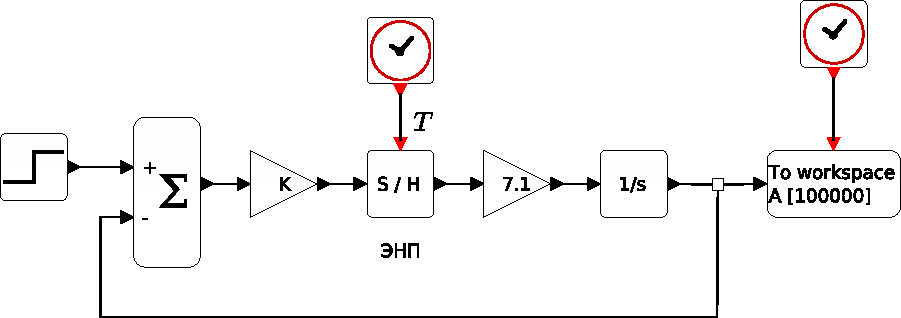
\includegraphics[width=0.7\textwidth]{scheme.pdf}
    \caption{Схема моделирования простенького ОУ.}
    \label{figure_just_example}
\end{figure}


\subsubsection{Вставка таблиц}\label{part_pasting_of_tables}
Пример оформления таблицы~--- см.~ниже по тексту.

\begin{table}[h]
    \caption{Параметры Денавита-Хартенберга.}
    \begin{tabular}{|c|c|c|c|c|}
        \hline
        Звено & $a_i$ & $\alpha_i$ & $d_i$ & $\theta_i$\\
        \hline
        1 & 0 & $\pi/2$ & $l_1$ & $\varphi_1+\pi/2$\\
        \hline
        2  & $l_2$ & $\pi$ & $s_1-2r$ & $\varphi_2-\pi/2$\\
        \hline
        3 & $l_3$ & $-\pi/2$ & $s_2-2r$ & $-\varphi_3$\\
        \hline
        4 & $l_4$ & $-\pi/2$ & $s_3-2r$ & $-\varphi_4$\\
        \hline
        5 & $l_5$ & $-\pi/2$ & $s_4-2r$ & $-\varphi_5$\\
        \hline
        6 & $l_6$ & $-\pi/2$ & $s_5-2r$ & $-\varphi_6$\\
        \hline
    \end{tabular}
    \label{table_DH_params}
\end{table}


\subsubsection{Вставка формул}\label{part_pasting_of_formulas}
Пример оформления формулы:
\begin{equation}\label{eq_example_of_formula}
    W(s) = \cfrac{T_ms+1}{T_ms^2+T_es+1}
\end{equation}
где $T_m$~--- первая постоянная, а $T_e$~--- вторая.


\subsection{Числовые данные ссылок}\label{part_editing_of_refs}
Ссылка на раздел~--- \ref{part_example_of_doc_inside}.
Ссылка на подраздел~--- \ref{part_pasting_of_extra_objects}.
Ссылка на что-то меньшее подраздела~--- \ref{part_pasting_of_figures}.
Cсылка на приложение~--- \ref{append_app_example}.
Ссылка на рисунок~--- \ref{figure_just_example}.
Ссылка на таблицу~--- \ref{table_DH_params}.
Ссылка на формулу~--- \eqref{eq_example_of_formula}.
Ссылка на источник~--- \cite{UrcolaIROS08}\footnote{Описание описания источника~--- см.~used\_books.bib.}.
\newpage
    \section*{Заключение}
\addcontentsline{toc}{section}{Заключение}
Текст заключения
\newpage
    \renewcommand\refname{Список использованных источников}
    \bibliography{used_books}
    \ESKDappendix{обязательное}{Название приложения}\label{append_app_example}
Текст приложения
\end{document}